%=======================================================================
%  3.2 CREATING  (text from the Word report; audit edits only)
%=======================================================================
\subsection{Creating: Engineering Concept Development}
\label{sec:creating}

\subsubsection{Structured Ideation: Crazy 8s}
\label{sec:crazy8}

Table~\ref{tab:crazy8} translates the biological mechanisms in
Section~\ref{sec:discovering} into eight technical building blocks.

\begin{table}[!htb]
\centering
\caption{Crazy 8s building blocks, before concept combinations.}
\label{tab:crazy8}
\renewcommand{\arraystretch}{1.15}
\small
\begin{tabularx}{\textwidth}{L{2.8cm} L{0.9cm} L{4.1cm} X}
\toprule
\textbf{Idea} & \textbf{Fn.} & \textbf{Biological starting point} & \textbf{Technical building block} \\
\midrule
1 Fixed shade & F2 & Cactus ribs change exposure. & Projecting ribs shade the façade. \\
2 Conductive fins & F3 & Elephant hairs act as small fins. & Separated projections conduct heat to air. \\
3 Surface texture & F3 & Sparse hairs suggest distributed structures. & Small roughness elements alter near-wall airflow. \\
4 Solar reflector & F1 & Silver-ant hairs reflect sunlight. & A reflective coating reduces solar absorption on a façade or roof. \\
5 Infrared emitter & F3 & Silver-ant hairs enhance thermal emission. & A sky-facing surface releases infrared heat. \\
6 Fluid transport & F3 & Blood carries heat to jackrabbit ears. & A fluid carries heat to a separate exchange surface. \\
7 Variable exchange area & F3 & Ear blood flow regulates heat release. & Connect more exchange area when cooling demand rises. \\
8 Responsive shade & F2 & Unequal swelling bends pine-cone scales. & A humidity-responsive layer changes shade position. \\
\bottomrule
\end{tabularx}
\end{table}

\needspace{15\baselineskip}
\subsubsection{Combining Ideas with a Morphological Matrix}
\label{sec:morph}

Table~\ref{tab:morph} groups alternatives by function. Bracketed numbers refer to
Table~\ref{tab:crazy8}; Option 3 draws on further models from
Section~\ref{sec:discovering}.

\begin{table}[!htb]
\centering
\caption{Alternatives for heat shielding, reflection, heat transport and heat release.}
\label{tab:morph}
\renewcommand{\arraystretch}{1.15}
\small
\begin{tabularx}{\textwidth}{L{3.0cm} X X X}
\toprule
\textbf{Design choice} & \textbf{Option 1} & \textbf{Option 2} & \textbf{Option 3} \\
\midrule
S -- Heat shielding & Fixed ribs (1) & Responsive louvers (8) & Insulating outer layer (camel fur) \\
O -- Solar reflection & Reflective roof (4) & Reflective façade (4) & Multilayer reflector (Morpho wings) \\
T -- Heat transport & Fluid loop (6) & Conduction through texture (2/3) & Fan-driven air cavity (bee fanning) \\
E -- Heat release & Roof emitter (5) & Wall exchange with local air and sky & Evaporating wet layer (camel sweat) \\
\bottomrule
\end{tabularx}
\end{table}

\textbf{A = S1--O1--T1--E1} combines fixed fins, a reflective roof and a water loop.
\textbf{B = T2--E2} uses a textured coating for local heat exchange.
\textbf{C = S2--O2--E2} combines responsive louvers with a reflective façade.
Variable connected area (7) remains an unselected regulation option for
\textbf{A}.

Camel fur limits heat gain and sweating removes heat by evaporation, suggesting an
insulating outer layer and a wet cooling surface~\cite{schmidtnielsen1957}. Morpho
wing structures suggest a multilayer reflector, although solar cooling requires
separate verification~\cite{giraldo2016}. Bee fanning suggests temperature-switched
fans moving air through a cavity~\cite{peters2019}. These options were not developed
further because of water or power demand, uncertain optical performance, or
insulation restricting outward heat transfer.

\textbf{C} was set aside because humidity does not directly indicate cooling demand.
Reflective façades also increased pedestrian heat stress in simulations of a
Stuttgart street canyon~\cite{lee2018}. \textbf{A} therefore places its reflective
surface on the roof. \textbf{A} and \textbf{B} were retained for the engineering
comparison below.

\subsubsection{Concept A V1 --- Water Façade}
\label{sec:conceptA}

\textbf{A} V1 was conceived for a new building, with water pipes in an absorber layer
in front of the wall and timber fins providing shade (Figure~\ref{fig:conceptA}).
The water loop carries residual heat to a separate roof surface for release. V1 has
no access panels in front of the pipes and the fins reach the ground; both points
are changed in V2 (Section~\ref{sec:v2}).

\begin{figure}[htbp]
\centering
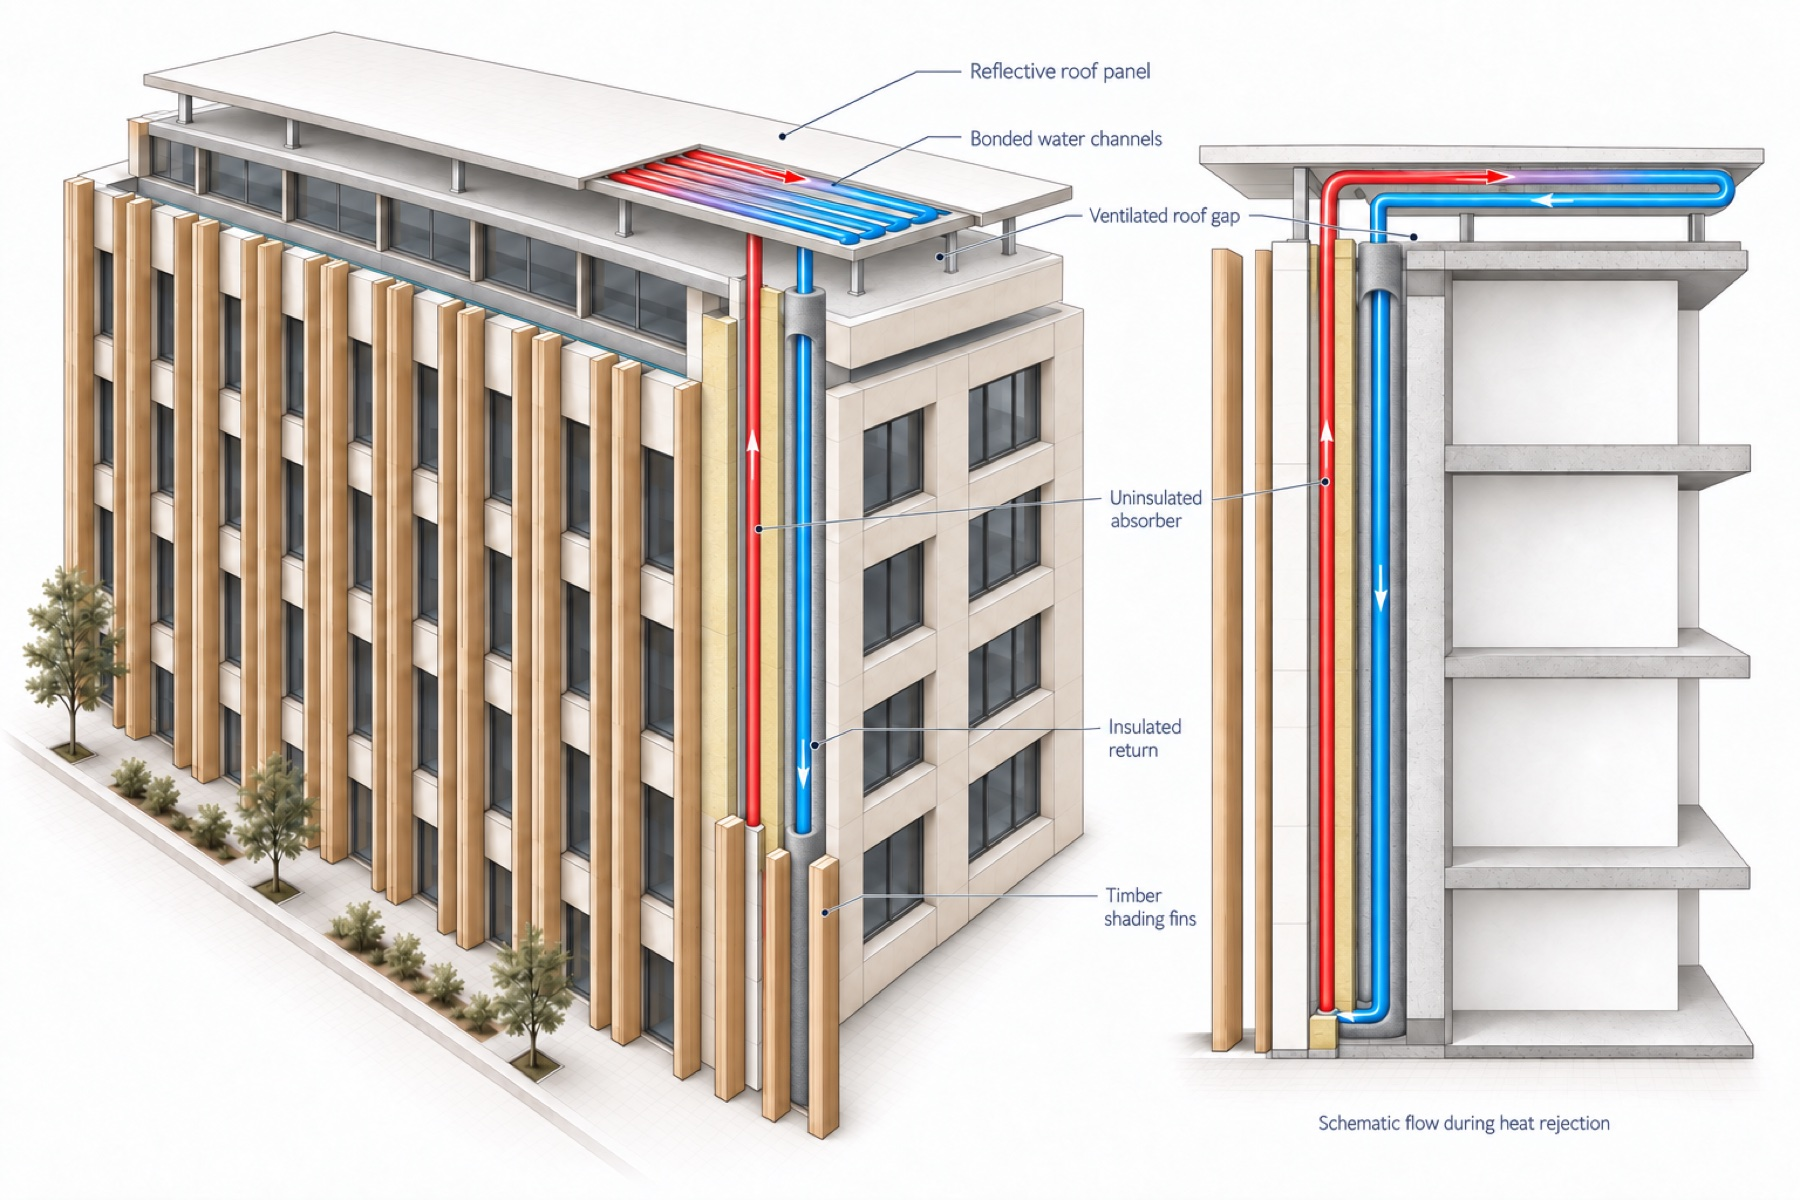
\includegraphics[width=0.85\textwidth]{figures/image6.jpg}
\caption{Concept A V1. Timber ribs shade the façade; water carries residual heat to
the roof and returns after cooling. Drawing: project team.}
\label{fig:conceptA}
\end{figure}

Cactus ribs inspire shading~\cite{lewis1977}; blood flow to jackrabbit ears inspires
heat transport to a separate exchange surface~\cite{asknature_jackrabbit}. Warmer
water can rise and cooler water return if buoyancy overcomes pipe
resistance~\cite{akhter2021}.

\subsubsection{Concept B V1 --- Roughness Spray Retrofit}
\label{sec:conceptB}

\textbf{B} V1 is a retrofit coating for an existing wall. Elephant hairs suggest
small heat-transfer structures, but work as conductive fins~\cite{myhrvold2012}. The
spray instead aims to disturb warm near-wall air (Figure~\ref{fig:conceptB}). Its
benefit depends on texture size, spacing, conductivity and local wind.

\begin{figure}[htbp]
\centering
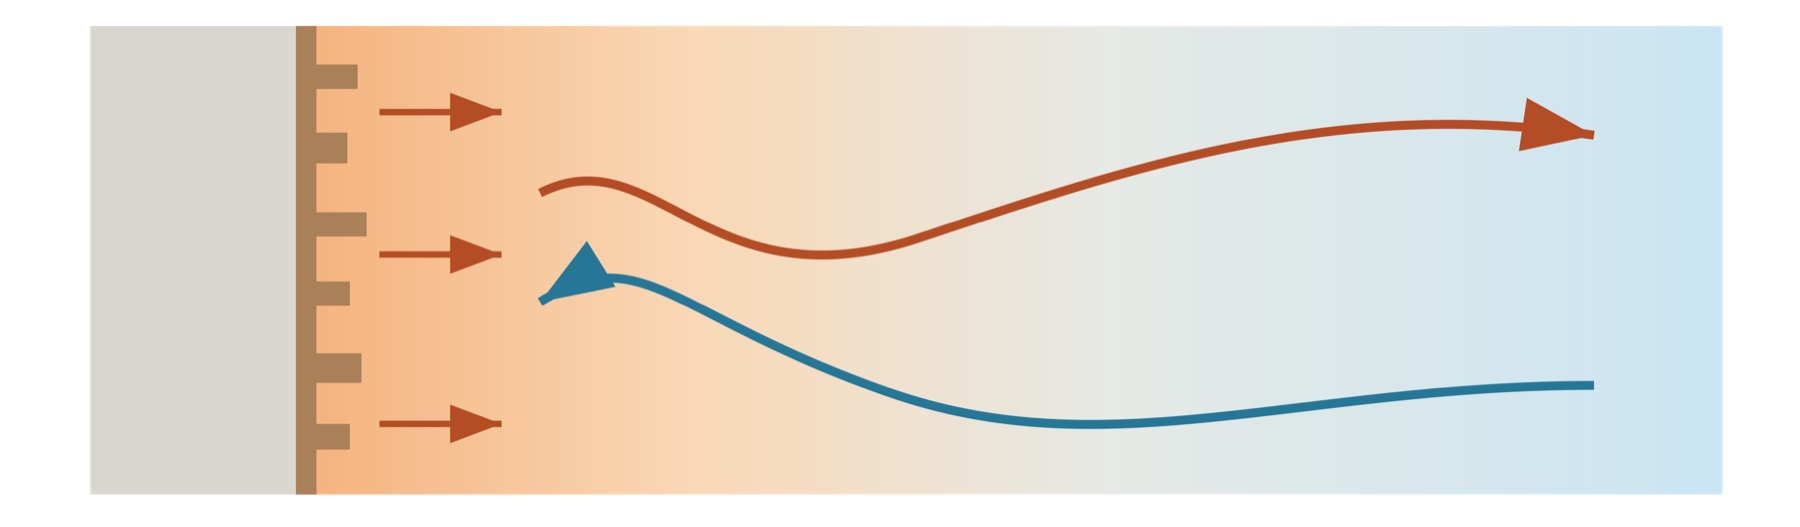
\includegraphics[width=\textwidth]{figures/image7.jpg}
\caption{Proposed roughness mechanism. Orange: warm near-wall air (thermal boundary
layer); blue: cooler surrounding air, with a gradual temperature transition.
Straight arrows: heat from the wall. Curved arrows: proposed air exchange; its
cooling benefit requires testing. Drawing: project team.}
\label{fig:conceptB}
\end{figure}

The build-up we propose is, from the wall outward, the existing rendered wall, a
mineral primer for adhesion, and a textured top coat \qtyrange{2}{4}{\milli\metre}
thick that carries sparse protruding elements. The element geometry follows the
density argument of Myhrvold et al.~\cite{myhrvold2012}: dense structures trap air
and insulate, sparse ones act as fins. We therefore assume elements
\qtyrange{5}{15}{\milli\metre} high at a centre spacing of
\qtyrange{20}{40}{\milli\metre}. Candidate materials are a silicate or lime-cement
binder with quartz or expanded-glass granules as the protruding elements. The
conductivity of the granule matters less than the disturbance of the near-wall air,
because the wall itself supplies the heat. The chemistry of binder and granules is
open and belongs to the material checks of Section~\ref{sec:priorities}.

To give \textbf{B} a number of the same kind as \textbf{A} we made an
order-of-magnitude estimate. On a vertical wall in still air the natural-convection
coefficient is about $h \approx \qtyrange{3}{5}{\watt\per\square\metre\per\kelvin}$;
façade coefficients in this range appear at low wind in the CFD study of Blocken et
al.~\cite{blocken2009}, and the order follows from the free-convection correlations
in White~\cite{white2011}. Myhrvold et al.~\cite{myhrvold2012} measured up to
\qty{23}{\percent} more heat loss from sparse hairs at low wind. If the texture
reaches the same enhancement, the added coefficient is
$\Delta h \approx \qty{1}{\watt\per\square\metre\per\kelvin}$. The extra heat
removed is
\begin{equation}
\Delta \dot{Q} = \Delta h \, A \, \Delta T
  \approx \qty{1}{\watt\per\square\metre\per\kelvin} \times \qty{1220}{\square\metre}
  \times \qty{10}{\kelvin} \approx \qty{12}{\kilo\watt},
\end{equation}
with $A$ the connected façade area of Table~\ref{tab:assumptions} and $\Delta T$ an
assumed wall-to-air difference of \qty{10}{\kelvin} on a hot afternoon. The estimate
assumes still air; wind would raise both the base coefficient and the absolute gain.
It also assumes the sign of the effect: Ahmed and Tanda~\cite{ahmed2024} found that
transverse ribs on a vertical surface can reduce laminar natural convection, so
whether a given texture helps or hurts depends on its geometry and must be measured.
If the mechanism works, \textbf{B} could remove roughly a quarter of the
\qty{44}{\kilo\watt} that \textbf{A}'s roof can release
(Section~\ref{sec:v2check}), with a few millimetres of coating instead of pipes,
panels and a roof plate. Section~\ref{sec:kpicompare} uses this figure.

\needspace{10\baselineskip}
\subsubsection{Engineering Canvas}
\label{sec:canvas}

{\small
\renewcommand{\arraystretch}{1.15}
\begin{longtable}{L{2.5cm} L{6.1cm} L{6.1cm}}
\caption{Engineering Canvas for the two V1 concepts.}
\label{tab:canvas}\\
\toprule
\textbf{Canvas item} & \textbf{A V1 --- water façade} & \textbf{B V1 --- roughness spray} \\
\midrule
\endfirsthead
\toprule
\textbf{Canvas item} & \textbf{A V1 --- water façade} & \textbf{B V1 --- roughness spray} \\
\midrule
\endhead
\bottomrule
\endfoot
Function & Prevent heat gain; transport and release residual heat. & Increase local heat exchange with a thin retrofit. \\
Biological principle & Cactus shading; blood-borne heat transport; silver-ant optical properties. & Sparse elephant hairs provide distributed heat-transfer structures. \\
Technical transfer & Shade, conduct heat into water, circulate by buoyancy, release it at a reflective roof emitter. & Conduct heat into a texture and test its effect on airflow. \\
Components / materials & Timber ribs, collector, pipes, roof plate/coating, insulated return, expansion vessel and vents. & Existing wall, coating binder and textured particles (parameters in Section~\ref{sec:conceptB}); chemistry remains open. \\
Inputs / outputs & Sunlight and temperature difference $\rightarrow$ reflected light and roof heat release. Water recirculates. & Sunlight and airflow $\rightarrow$ heat exchange with local air and sky. \\
Requirements / KPIs & Section~\ref{sec:kpi} KPIs; little auxiliary energy; winter operation, glare and townscape constraints. & Same KPIs; thin application, adhesion and safe weathering. \\
Critical assumptions & Enough heat reaches the water; roof capacity and buoyancy are sufficient. & Texture improves heat transfer without trapping still air. \\
Uncertainties & Pipe resistance, roof output, leakage, frost and panel-to-pipe contact. & Cooling benefit, soiling, adhesion and weathering. \\
Next check & Estimate circulation and roof capacity. & Compare smooth and textured samples under the same wind and temperatures. \\
\end{longtable}}

\subsubsection{Critical Engineering Questions}
\label{sec:questions}

Q1: Can buoyancy circulate enough water? Q2: Can the roof release the collected
heat? Q3: Does the spray improve heat transfer under weak airflow?

\needspace{18\baselineskip}
\subsubsection{Engineering Check 1 --- Circulation and Pipe Size}
\label{sec:check1}

The first estimate applies \textbf{A} V1 to a hypothetical new building with the
dimensions of the Modellierungsgebiet 03 reference block.
Table~\ref{tab:assumptions} lists the model inputs and engineering assumptions; the
building dimensions were measured on our model of the reference block.

\begin{table}[!htb]
\centering
\caption{Assumptions for the circulation estimate.}
\label{tab:assumptions}
\renewcommand{\arraystretch}{1.15}
\small
\begin{tabularx}{\textwidth}{L{3.2cm} X}
\toprule
\textbf{Input} & \textbf{Value and basis} \\
\midrule
Building and façade & $64 \times \qty{58}{\metre}$ outer plan; $42 \times \qty{36}{\metre}$ courtyard; eaves at \qty{15.4}{\metre} and roof rise \qty{4}{\metre}. Two faces, assumed \qty{65}{\percent} opaque: Area $= (64 + 58) \times 15.4 \times 0.65 \approx \qty{1220}{\square\metre}$. \\
Collected heat & Assume $q'' = \qty{100}{\watt\per\square\metre}$ enters the water after shading; test \qtyrange{50}{150}{\watt\per\square\metre}. Collection depends on panel-to-pipe contact. \\
Height $H$ & Assume \qty{10}{\metre} between centres of heat collection and release. \\
Water near \qty{30}{\celsius} & Density $\rho \approx \qty{996}{\kilo\gram\per\cubic\metre}$; heat capacity $c_p \approx \qty{4180}{\joule\per\kilo\gram\per\kelvin}$; expansion coefficient $\beta \approx \qty{3.0e-4}{\per\kelvin}$~\cite[Table~3]{harvey1998}. Assume viscosity $\mu = \qty{0.8}{\milli\pascal\second}$. \\
Common pipe route & Assume smooth pipe, $L = \qty{160}{\metre}$, fitting-loss factor $\sum K = 20$~\cite{white2011}. Extra branch and radiator losses are excluded. \\
\bottomrule
\end{tabularx}
\end{table}

The chosen water-temperature differences, \qty{10}{\celsius} and \qty{3}{\celsius},
test stronger and weaker driving conditions. A smaller difference weakens buoyancy
while requiring more flow to carry the same heat load.

Heat rate $\dot{Q}$ is energy carried per second; $\dot{m}$ is water mass flow.
Assume steady liquid flow and approximate the hot/cold leg difference by the water
temperature change $\Delta T$:
\begin{align}
\dot{Q} &= A_\mathrm{f}\, q'' \approx \qty{1220}{\square\metre} \times
  \qty{100}{\watt\per\square\metre} = \qty{122}{\kilo\watt}, \label{eq:load}\\
\dot{m} &= \frac{\dot{Q}}{c_p\, \Delta T}; \qquad
\Delta p_\mathrm{b} \approx \rho\, g\, H\, \beta\, \Delta T, \label{eq:buoyancy}\\
\Delta p_\mathrm{loss} &= \left( f \frac{L}{D} + \sum K \right) \frac{\rho v^2}{2};
  \qquad v = \frac{4 \dot{m}}{\rho \pi D^2}. \label{eq:loss}
\end{align}
Here $D$ is internal diameter, $v$ water speed and $g = \qty{9.81}{\metre\per\square\second}$.
Use Darcy friction factor $f = 0.3164/\mathrm{Re}^{0.25}$, with
$\mathrm{Re} = \rho v D/\mu$~\cite{white2011}, and solve where friction equals
buoyancy~\cite{akhter2021}. $\mathrm{Re} \approx \numrange{26000}{39000}$ supports
the smooth-pipe turbulent-flow approximation.

\begin{table}[!htb]
\centering
\caption{Circulation estimates for the \qty{122}{\kilo\watt} load.}
\label{tab:circulation}
\renewcommand{\arraystretch}{1.15}
\small
\begin{tabular}{llll}
\toprule
\textbf{Water difference} & \textbf{Buoyancy pressure} & \textbf{Water flow} & \textbf{Internal diameter} \\
\midrule
\qty{10}{\celsius} (= \qty{10}{\kelvin}) & $\approx\qty{300}{\pascal}$ & \qty{2.9}{\kilo\gram\per\second} & $\approx\qty{180}{\milli\metre}$ \\
\qty{3}{\celsius} (= \qty{3}{\kelvin}) & $\approx\qty{90}{\pascal}$ & \qty{9.7}{\kilo\gram\per\second} & $\approx\qty{400}{\milli\metre}$ \\
\bottomrule
\end{tabular}
\end{table}

Reducing the temperature difference more than doubles the required main-pipe
diameter. These estimates use the whole available buoyancy pressure, because the
diameter was solved for friction equal to buoyancy; radiator, collector and fitting
losses need a budget of their own (Section~\ref{sec:v2check}). Varying the assumed
heat input from 50 to \qty{150}{\watt\per\square\metre} gives a load of
\qtyrange{61}{183}{\kilo\watt}.

\subsubsection{Engineering Check 2 --- Roof Heat Release}
\label{sec:check2}

In steady operation, the roof must release the heat collected by the façade. Raman
et al.~\cite{raman2014} measured \qty{40.1}{\watt\per\square\metre} net cooling at
air temperature under sunlight above \qty{850}{\watt\per\square\metre}. This
specialised emitter is used as a benchmark only.
\begin{equation}
A_\mathrm{release} = \dot{Q} / q''_\mathrm{net}
\end{equation}
For the engineering estimate, assume a \qty{35}{\celsius} roof, \qty{30}{\celsius}
air, effective sky temperature \qty{20}{\celsius}, solar reflectance $r = 0.95$,
thermal emittance $\varepsilon = 0.90$, sunlight $G = \qty{800}{\watt\per\square\metre}$
and convection coefficient $h = \qtyrange{3}{8}{\watt\per\square\metre\per\kelvin}$.
Effective sky temperature represents incoming infrared radiation, not air
temperature. Neglect back-surface exchange and assume an unobstructed sky:
\begin{equation}
q''_\mathrm{net} = h\,(T_\mathrm{roof} - T_\mathrm{air})
  + \varepsilon \sigma \left(T_\mathrm{roof}^{4} - T_\mathrm{sky}^{4}\right)
  - (1 - r)\, G. \label{eq:roof}
\end{equation}
The terms represent heat to air, infrared heat exchange and absorbed sunlight. With
$\sigma = \qty{5.67e-8}{\watt\per\square\metre\per\kelvin\tothe{4}}$, net release is
$15\text{--}40 + 83 - 40 \approx \qtyrange{58}{83}{\watt\per\square\metre}$. Roof tilt
and nearby buildings would change this estimate. This is a daytime case
($G = \qty{800}{\watt\per\square\metre}$); a night case has not been calculated.

\begin{table}[!htb]
\centering
\caption{Roof cooling area required to release the assumed \qty{122}{\kilo\watt} load.}
\label{tab:roofarea}
\renewcommand{\arraystretch}{1.15}
\small
\begin{tabular}{lll}
\toprule
\textbf{Case} & \textbf{Net heat release} & \textbf{Roof area for \qty{122}{\kilo\watt}} \\
\midrule
Published emitter benchmark & \qty{40.1}{\watt\per\square\metre} & $\approx\qty{3050}{\square\metre}$ \\
Assumed \qty{35}{\celsius} roof, \qty{20}{\celsius} sky & \qtyrange{58}{83}{\watt\per\square\metre} & $\approx$ \qtyrange{1470}{2100}{\square\metre} \\
Same roof, warmer \qty{30}{\celsius} sky & \qtyrange{4}{29}{\watt\per\square\metre} & $\approx$ \qtyrange{4200}{29500}{\square\metre} \\
\bottomrule
\end{tabular}
\end{table}

The model allocates about \qty{740}{\square\metre} to cooling: \qty{168}{\metre}
total strip width $\times$ \qty{4.39}{\metre} combined slope depth. Solar panels,
rooflights and gaps limit this area (Figure~\ref{fig:refblock}). The first two cases
give about \qtyrange{30}{62}{\kilo\watt}, supporting roughly
\qtyrange{300}{620}{\square\metre} of façade at \qty{100}{\watt\per\square\metre}. A
warmer sky reduces radiative heat loss; near-zero net output makes the required area
highly sensitive. The connected façade area must therefore be reduced.

\begin{figure}[htbp]
\centering
\begin{minipage}[t]{0.46\textwidth}
\centering
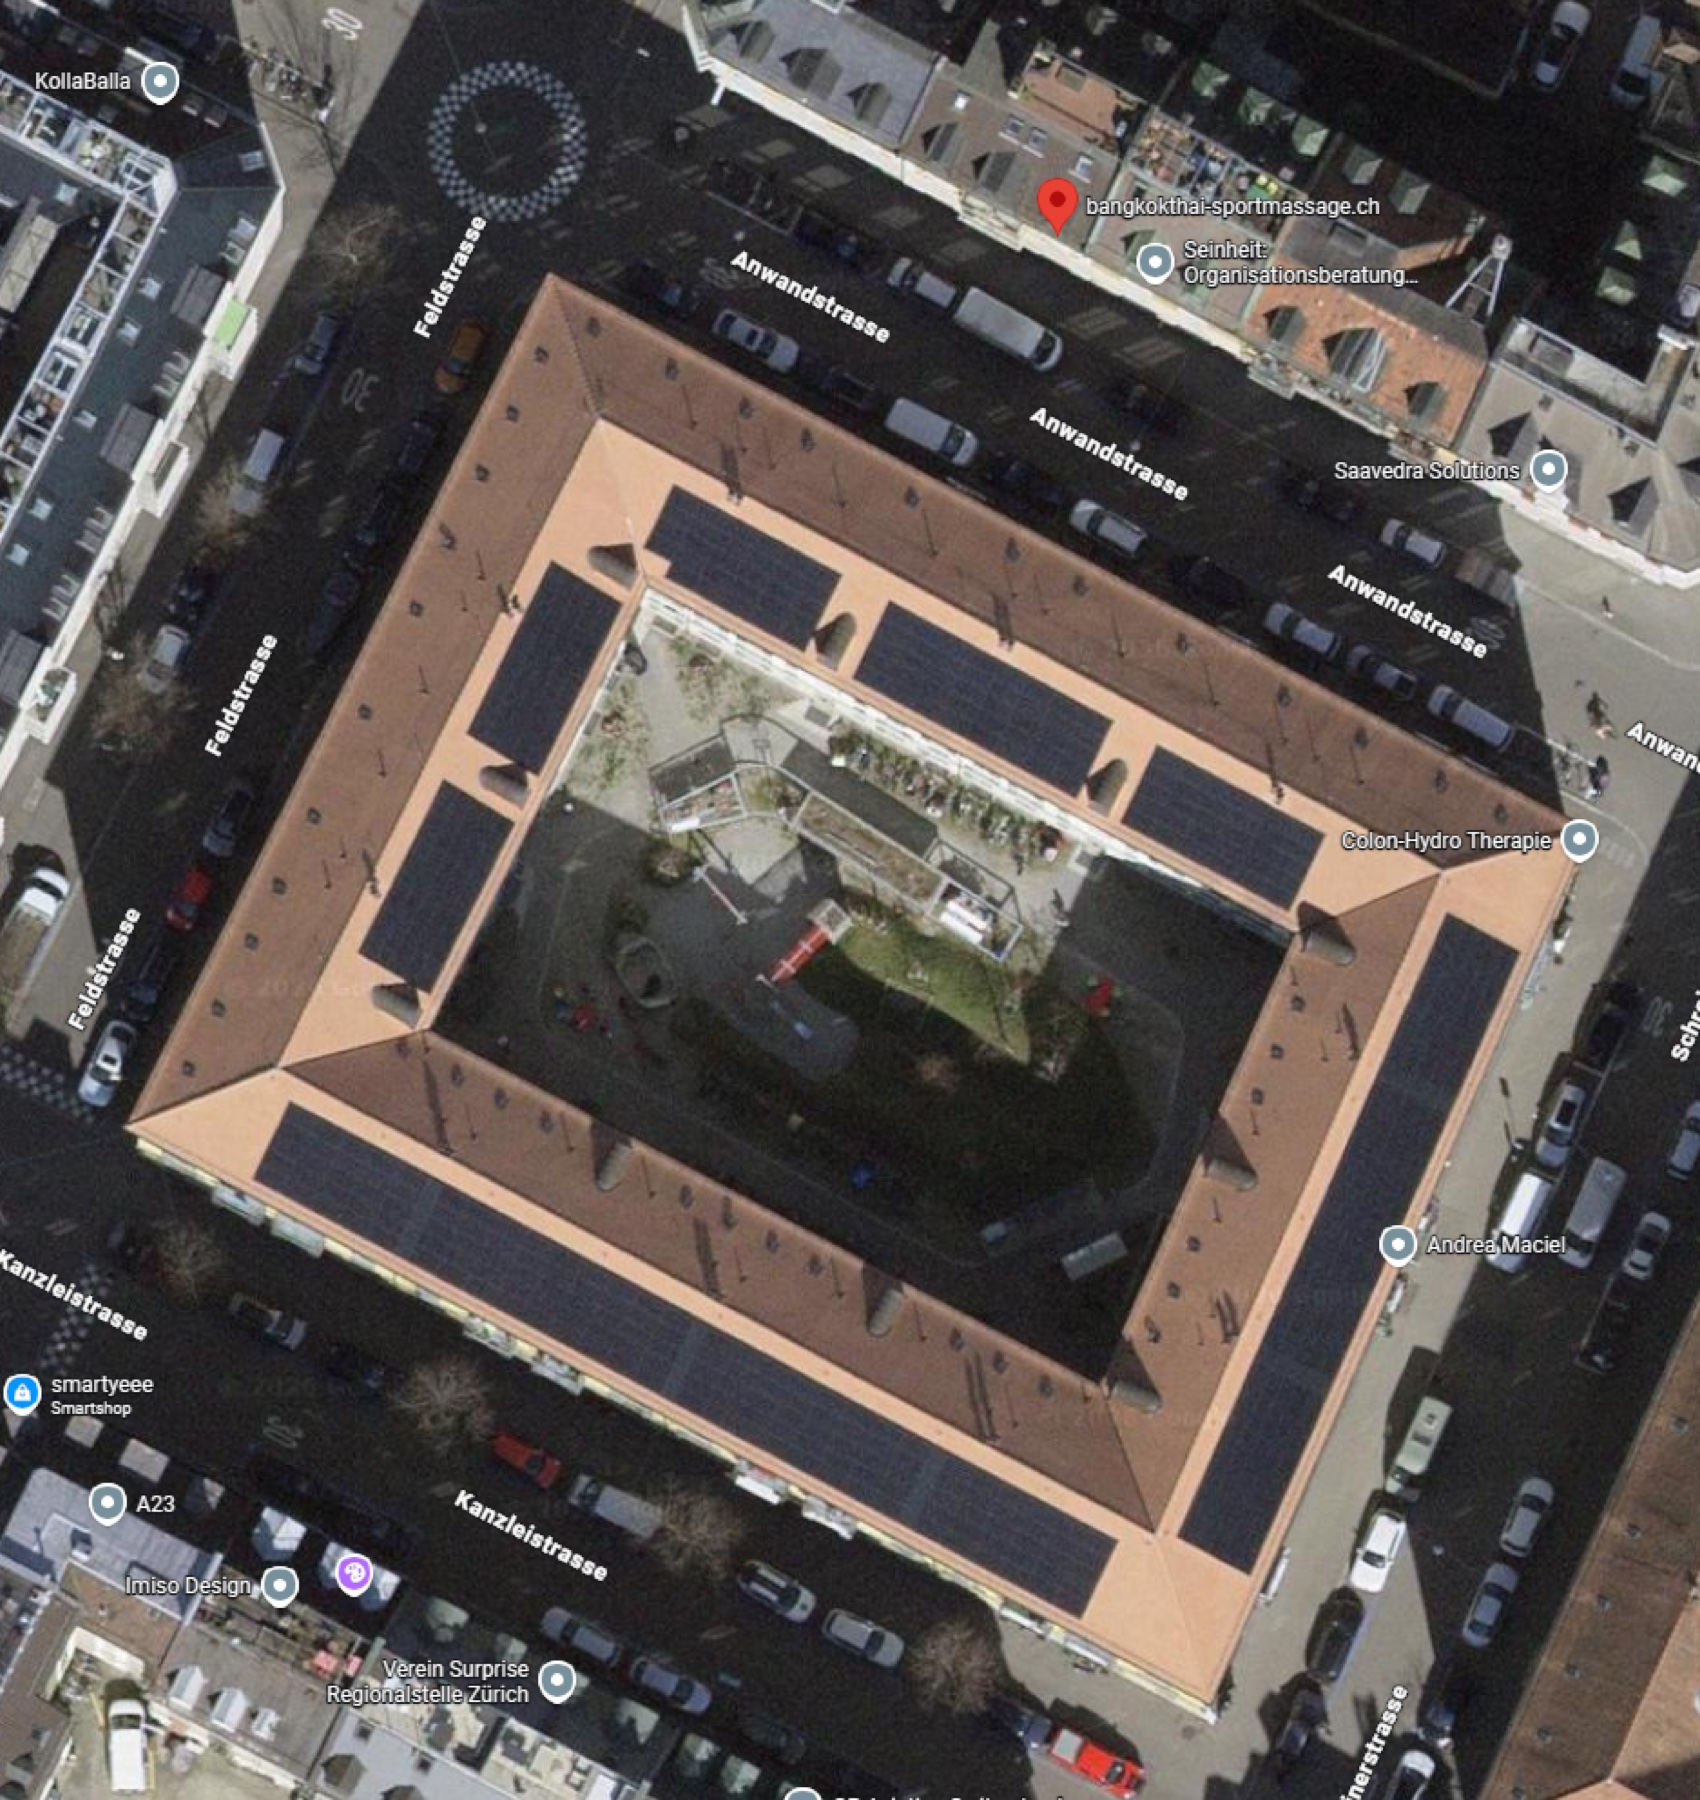
\includegraphics[width=\linewidth]{figures/image8.jpg}\\[1mm]
{\small (a) Reference building --- Google Maps}
\end{minipage}\hfill
\begin{minipage}[t]{0.50\textwidth}
\centering
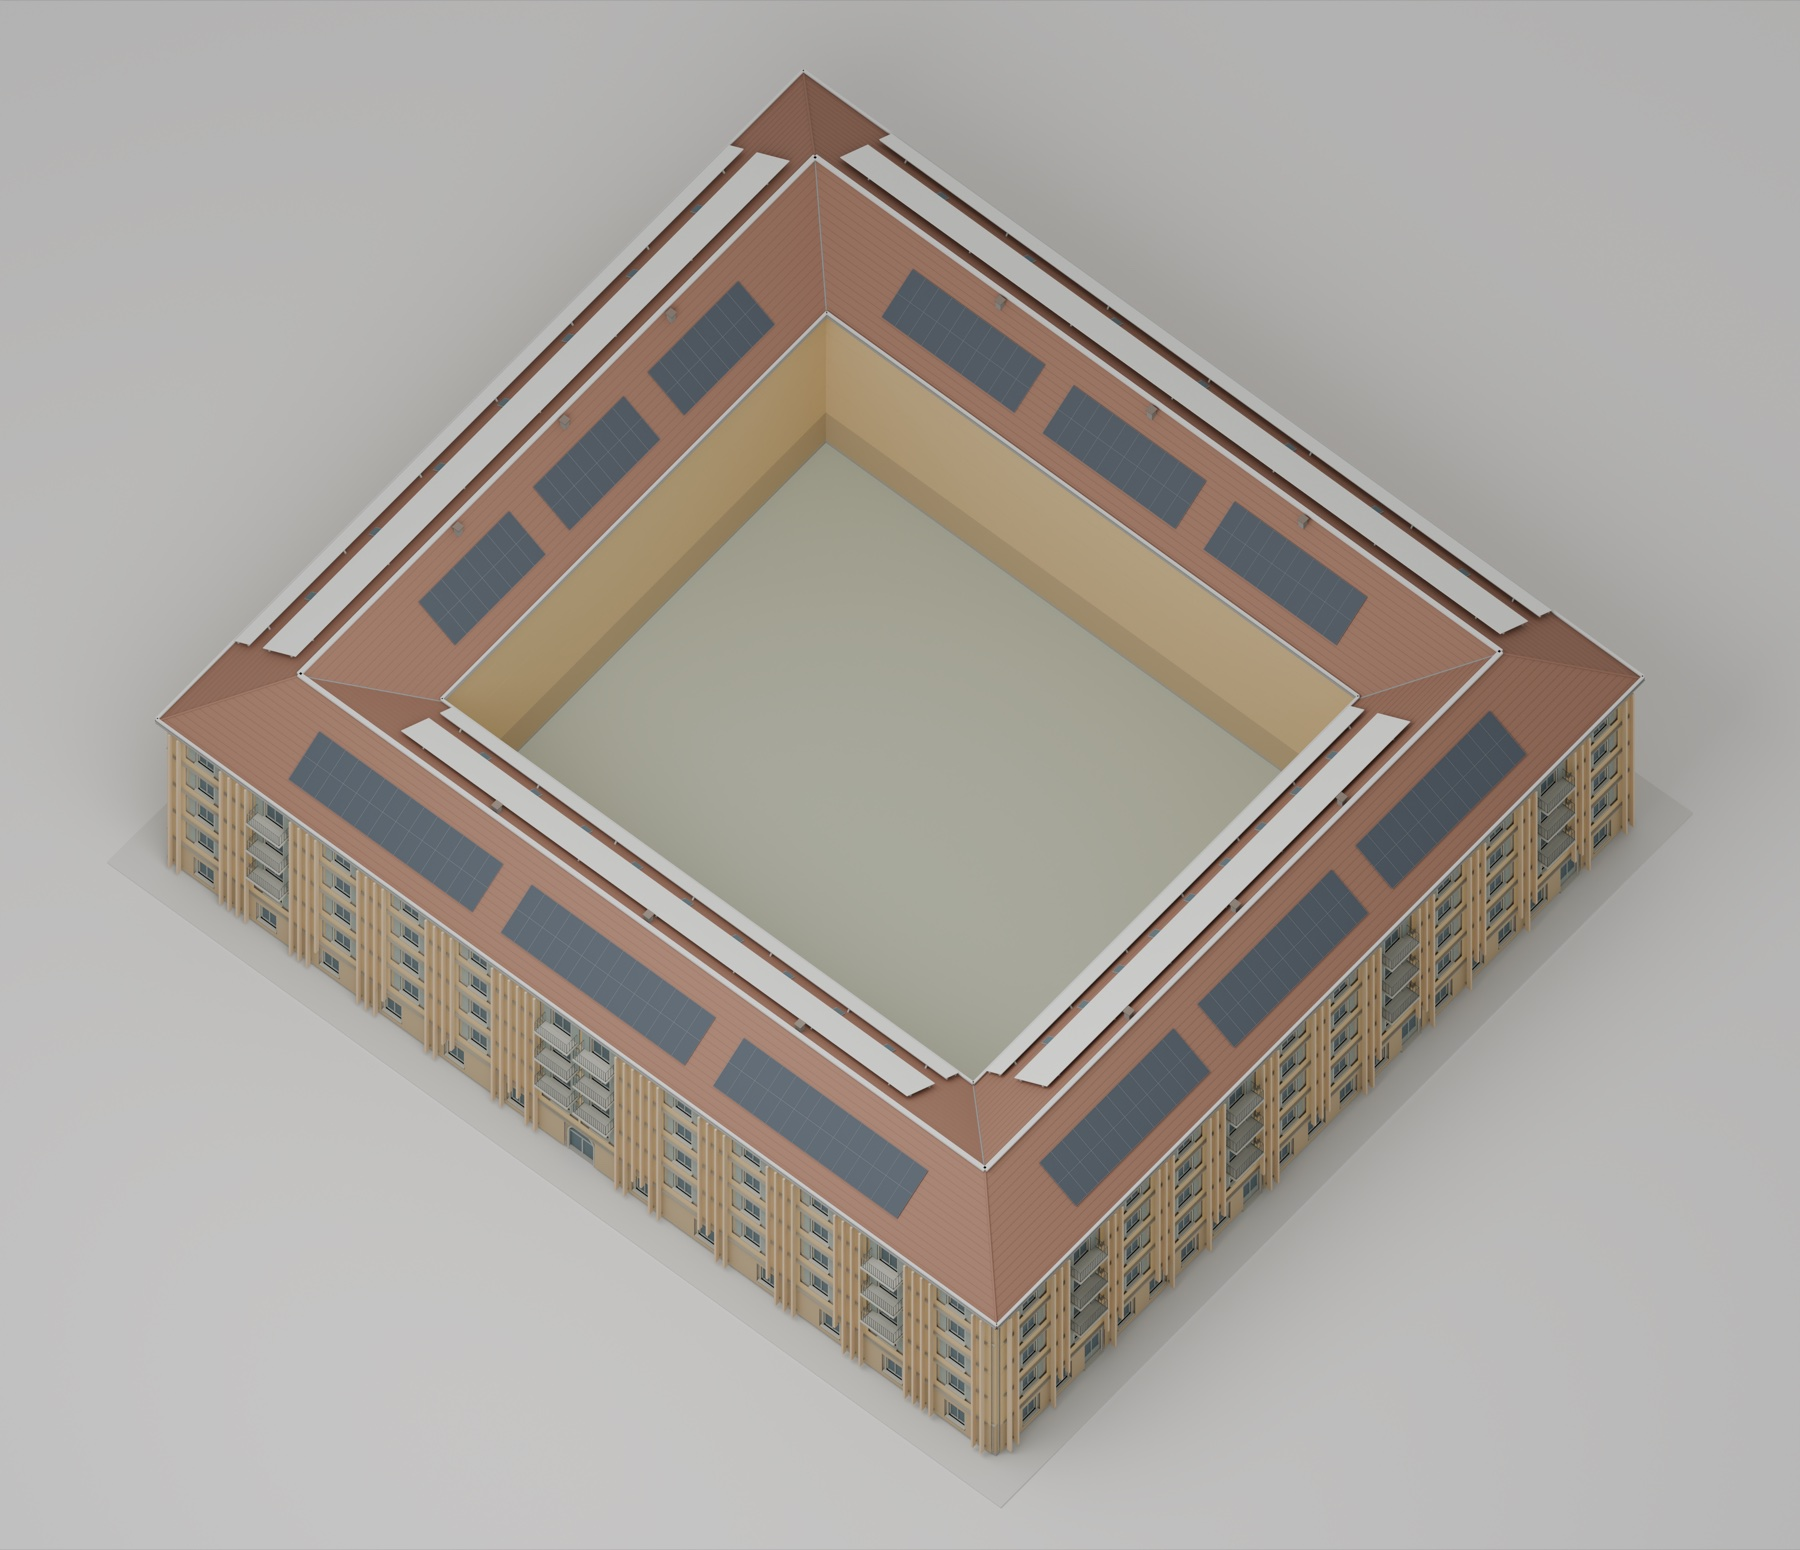
\includegraphics[width=\linewidth]{figures/image9.jpg}\\[1mm]
{\small (b) Proposed roof layout}
\end{minipage}
\caption{Reference Block in Modellierungsgebiet 03~\cite[pp.~148--151]{stadtzuerich2020}
and our model. Cooling strips share the roof with solar panels and rooflights.}
\label{fig:refblock}
\end{figure}
